\subsubsection{\stid{3.09} SLATE}\label{subsubsect:slate}


\paragraph{Overview}

The Software for Linear Algebra Targeting Exascale (SLATE) intends to
provide fundamental dense linear algebra capabilities
to the US Department of Energy (DOE)
and to the high-performance computing (HPC) community at large.
To this end, SLATE will provide
parallel Basic Linear Algebra Subprograms (BLAS),
linear systems solvers, least square solvers,
singular value and eigenvalue solvers.

The ultimate objective of SLATE is to replace the
venerable Scalable Linear Algebra PACKage (ScaLAPACK) library,
which has become the industry standard for dense linear algebra operations
in distributed-memory environments.
However, after two decades of operation,
ScaLAPACK is past the end of its life cycle and overdue for a replacement,
as it can hardly be retrofitted to support GPUs,
which are an integral part of today's HPC hardware infrastructure.

Primarily, SLATE aims to extract the full performance potential and maximum
scalability from modern HPC machines with large numbers nodes,
large numbers of cores per node, and multiple GPUs per node.
For typical dense linear algebra workloads, this means getting close
to the theoretical peak performance and scaling to the full size of the machine
(i.e., thousands to tens of thousands of nodes).
This is to be accomplished in a portable manner by relying mostly on standards
like MPI and OpenMP.

SLATE functionalities will first be delivered to the ECP applications
that most urgently require SLATE capabilities
(NWChem, GAMESS, EXAALT, QMCPACK, CANDLE, etc.)
and to other software libraries
that rely on underlying dense linear algebra services
(STRUMPACK, SuperLU, etc.).
Figure~\ref{fig:slate-architecture} shows the role of SLATE
in the ECP software stack.

While the initial objective of SLATE is to serve as a successful,
drop-in replacement for ScaLAPACK with support for GPU accelerators,
the ultimate goal of SLATE is to deliver dense linear algebra capabilities
way beyond the capabilities of ScaLAPACK.
The low-hanging fruits include implementation of more communication-avoiding
algorithms and randomization algorithms
(based on random projections and sampling).
Also within the reach of SLATE are features like:
support for variable size tiles, support for low-rank compressed tiles,
and possibly support for block-sparse matrices.

\begin{figure}[htb]
    \centering
    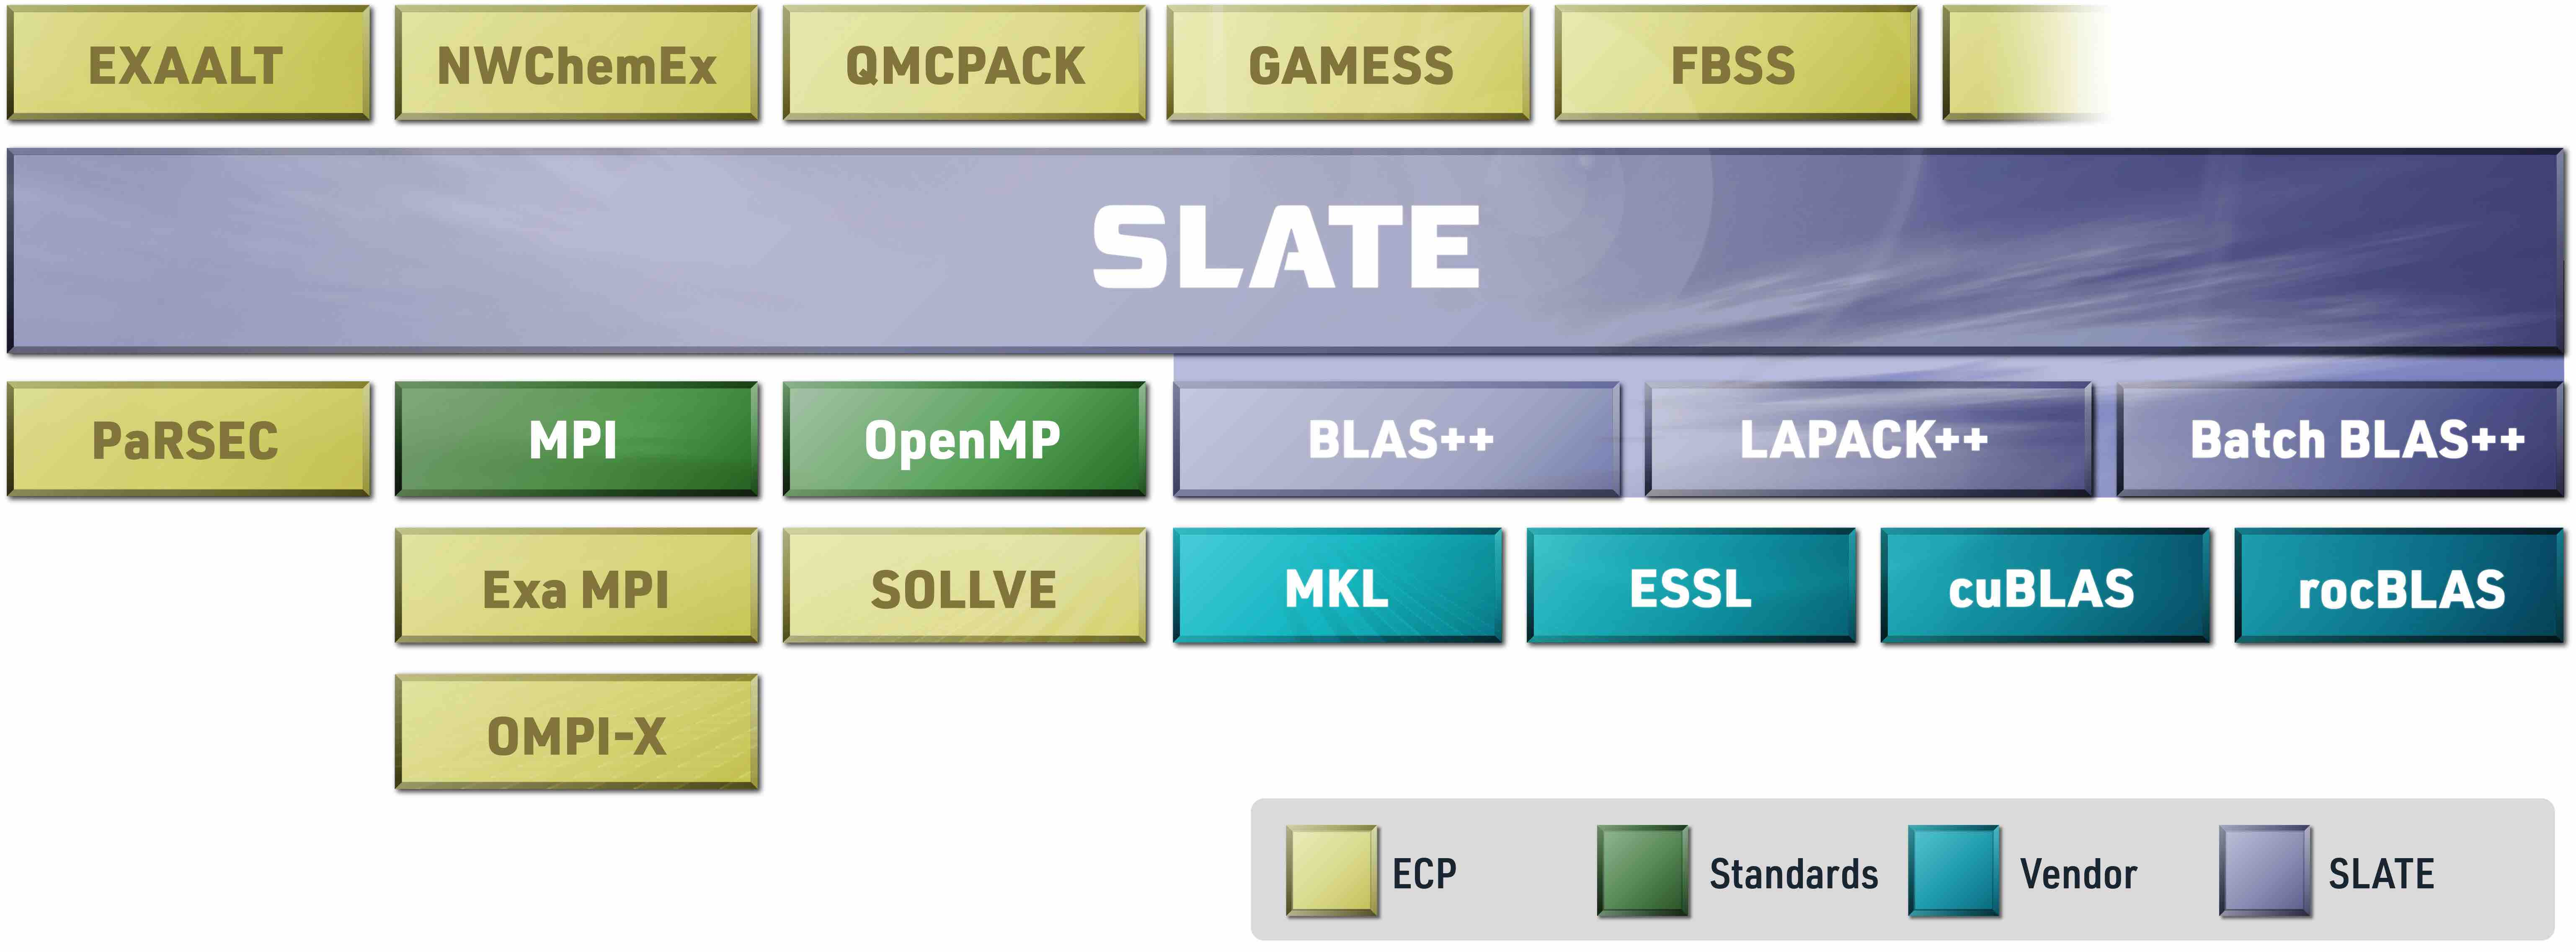
\includegraphics[width=0.75\textwidth]{projects/2.3.3-MathLibs/2.3.3.09-SLATE/SLATE-architecture.jpg}
    \caption{\label{fig:slate-architecture}
    SLATE in the ECP software stack.}
\end{figure}

\paragraph{Key  Challenges}

\begin{enumerate}
\item
\textbf{Designing from the ground up:}
The SLATE project's primary challenge stems from the need to design the package
from the ground up, as no existing software package offers
a viable path forward for efficient support of GPUs
in a distributed-memory environment.
\item
\textbf{Facing harsh hardware realities:}
SLATE is being developed in a harsh hardware environment, where virtually
all the processing power is on the GPU side.
Achieving efficiency requires very aggressive offload to GPU accelerators
and very careful optimization of multiple bottlenecks.
Being a distributed computing package, SLATE also faces the grim reality
of the interconnection technology lagging horribly behind the computing
capabilities of the GPUs.
\item
\textbf{Facing harsh software realities:}
SLATE is being developed using cutting-edge software technologies,
and relies on modern features of the C++ language and recent extensions
to the OpenMP standard, many of which are not fully supported by compilers
and their runtime environments.
In terms of GPU acceleration, standardized solutions are still in flux.
Also, while complete parallel programming frameworks exist, at this stage
they have to be considered research prototypes.
\end{enumerate}

\paragraph{Solution Strategy}

\begin{enumerate}
\item
\textbf{Evolving design:}
Due to the inherent challenges of designing a software package
from the ground up, the SLATE project started
with a careful analysis of the existing and emerging
implementation technologies~\cite{abdelfattah2017roadmap},
and followed with a phase
of laying out the initial design~\cite{kurzak2017designing}.
Since then, the team rolls out new computational routines every quarter,
while frequently refactoring and occasionally redesigning the underlying
software infrastructure.
\item
\textbf{Focus on GPUs:}
Efficient GPU acceleration is the primary focus of performance
engineering efforts in SLATE.
Where applicable, highly optimized vendor implementations of GPU operations
are used, such as the batch {\tt gemm} routine.
Where necessary, custom GPU kernels are developed, like in the case of computing
matrix norms.
Care is taken to hide communication to and from the GPUs by overlapping it with
execution of GPU computations.
\item
\textbf{Community engagement:}
The SLATE team interact on a regular basis with the OpenMP community,
represented in ECP by the SOLLVE project, and with the MPI community,
represented in ECP by the OMPI-X project and the Exascale MPI project.
The SLATE team also engages the vendor community through our contacts
at Intel, NVIDIA, AMD, and ARM.
\end{enumerate}

\paragraph{Recent Progress}

During each quarter of 2018, the SLATE team has been adding to its suite
by releasing new computational routines:
parallel Level 3 BLAS in March,
parallel norms in June,
linear systems solvers (LLT, LU, LDLT) in September,
and least squares solvers (CAQR/LQ) in December.
All routines are available in all standard precisions:
single real (S), single complex (C), double real (D), and double complex (Z),
all accompanied by appropriate testers.
In addition to SLATE's native, C++ API, compatibility APIs for LAPACK
and ScaLAPACK users are also provided, so that SLATE can serve
as a drop-replacement.
All developments are documented in SLATE Working Notes
\footnote{\url{http://www.icl.utk.edu/publications/series/swans}.}

\paragraph{Next Steps}

\begin{enumerate}
\item
\textbf{Mixed-precision Linear Solvers:}
We plan to implement mixed-precision linear solvers by the end of March 2019.
Mixed precision routines factor the matrix in lower precision, e.g., single,
and compute the linear system solution in higher precision, e.g., double,
in the process of iterative refinement.
In most cases, results in the high precision can be produced at the speed
of computing in the low precision.
The half precision of the Tensor Cores of the V100 GPUs are a possible target
of this technique.
\item
\textbf{Matrix Inversion Routines:}
We plan to implement matrix inversion routines by the end of June 2019.
Explicit matrix inverses are required by applications in computational
chemistry and statistics, and offer a high potential for optimization
by pipelining the different algorithmic steps.
Routines for inverting general, symmetric positive definite, and symmetric
indefinite matrices are planned.
\item
\textbf{SVD and EVP Solvers:}
We plan to implement SVD routines and symmetric EVP routines
by the end of September 2019.
The implementations will be based on state-of-the-art two-stage reductions
and divide-and-conquer algorithms.
Superior performance is expected, as well as strong benefit
from GPU acceleration.
\end{enumerate}
